\documentclass[12pt,a4paper,onecolumn]{exam}
\usepackage{amsmath}
\usepackage{amssymb}
\usepackage{graphicx}
\usepackage{float}
\usepackage{geometry}
\usepackage{tikz}
\usepackage[skins]{tcolorbox} % Use [skins] to get the rounded shape


% --- Define our simple \questionheader command ---
\newcommand{\questionheader}[1]{%
  \begin{tcolorbox}[
    enhanced,
    colback=black,
    coltext=white,
    boxrule=0pt,
    fontupper=\Large\bfseries,
    arc=4mm
  ]
  #1
  \end{tcolorbox}%
}
% --- End of definition ---
\newtcolorbox{answerbox}[1]{
  boxrule=0.4pt,   % Sets the thickness of the border
  colback=white,   % Sets the background color
  height=#1,       % <-- Use the first argument (#1) as the height
}


\usepackage[font = small]{caption}
\usepackage{subcaption}

\newenvironment{blanksolution}
  {%
    \renewcommand{\solutiontitle}{\noindent}%
    \begin{solution}%
  }%
  {\end{solution}}
\usepackage{listings}

\lstset{
    language=Python,
    basicstyle=\ttfamily,
    }

\pagestyle{headandfoot}
% \firstpageheader{Assignment 2}{}{Dwaipayan Haldar}
\runningheader{Assignment 3}{Detection and Estimation Theory}{Dwaipayan Haldar}


\begin{document}

\begingroup
    \centering
    \LARGE E1 244 Detection and Estimation Theory\\
    \LARGE Assignment 3\\[0.5em]
    \large Dwaipayan Haldar\par
    \large \today\\[0.5em] 
\endgroup
\noindent\rule{\textwidth}{0.5pt}
\printanswers
\renewcommand{\solutiontitle}{\noindent\textbf{Ans:}\enspace}



\questionheader{Problem 1}

\begin{solution}
\textbf{(a)} Let $T(Y)=|Y|$.

\textbf{(i)} Since $Y\in\{-1,0,1\}$, we have
\[
T\in\{0,1\}.
\]

\textbf{(ii)} The pmf is
\[
f(y;\theta)=\left(\frac{\theta}{2}\right)^{|y|}(1-\theta)^{1-|y|},\qquad y\in\{-1,0,1\}.
\]
Write it as
\[
f(y;\theta)=g(T(y),\theta)\,h(y),
\]
with
\[
g(t,\theta)=\left(\frac{\theta}{2}\right)^t(1-\theta)^{1-t},\qquad h(y)=1.
\]
Hence, by Neyman-Fisher factorization, $T(Y)=|Y|$ is sufficient.

\textbf{(iii)} Conditional distribution:
\[
P(Y=y\mid T=0)=
\begin{cases}
1,&y=0,\\
0,&\text{otherwise},
\end{cases}
\]
and
\[
P(Y=y\mid T=1)=
\begin{cases}
\frac12,&y=\pm1,\\
0,&\text{otherwise}.
\end{cases}
\]
So $f(y\mid T)$ does not depend on $\theta$.

\textbf{(iv)} Completeness: let $E_\theta[g(T)]=0$ for all $\theta\in[0,1]$. Then
\[
g(0)(1-\theta)+g(1)\theta=0,\quad \forall\theta.
\]
Putting $\theta=0$ gives $g(0)=0$, and $\theta=1$ gives $g(1)=0$. Hence $g(T)=0$ a.s., so $T$ is complete.

\vspace{0.5em}
\textbf{(b)} Estimator:
\[
\hat\theta(Y)=
\begin{cases}
2,&Y=1,\\
0,&\text{otherwise}.
\end{cases}
\]

\textbf{(i)} It is not very reasonable structurally, since it can take value $2$ while $\theta\in[0,1]$.

\textbf{(ii)} Unbiasedness:
\[
E_\theta[\hat\theta]=2P_\theta(Y=1)=2\cdot\frac{\theta}{2}=\theta.
\]

\textbf{(iii)} Variance:
\[
\operatorname{Var}_\theta(\hat\theta)=E_\theta[\hat\theta^2]-\theta^2
=4P_\theta(Y=1)-\theta^2
=2\theta-\theta^2.
\]

\vspace{0.5em}
\textbf{(c)} Rao-Blackwell improvement using $T$:
\[
\hat\theta_{\text{new}}(T)=E[\hat\theta\mid T].
\]
If $T=0$, then $Y=0$ so $\hat\theta=0$.
If $T=1$, then $Y=\pm1$ with probability $1/2$ each, so
\[
E[\hat\theta\mid T=1]=2\cdot\frac12+0\cdot\frac12=1.
\]
Therefore
\[
\hat\theta_{\text{new}}=
\begin{cases}
1,&T=1,\\
0,&T=0,
\end{cases}
=T=|Y|.
\]
Its variance:
\[
\operatorname{Var}_\theta(\hat\theta_{\text{new}})
=\operatorname{Var}_\theta(T)=\theta(1-\theta)=\theta-\theta^2.
\]
Comparison:
\[
\operatorname{Var}_\theta(\hat\theta)-\operatorname{Var}_\theta(\hat\theta_{\text{new}})
=(2\theta-\theta^2)-(\theta-\theta^2)=\theta\ge0,
\]
strictly smaller for $\theta>0$.
\end{solution}
\questionheader{Problem 2}

\begin{solution}
\textbf{Given:} $Y_1,Y_2\stackrel{\text{i.i.d.}}{\sim}\mathrm{Poisson}(\lambda)$, $\lambda>0$, and $\theta=e^{-\lambda}$.

\textbf{(a)} Let $T=Y_1+Y_2$. Using mgf:
\[
M_{Y_i}(t)=\exp\{\lambda(e^t-1)\},
\]
so
\[
M_T(t)=M_{Y_1}(t)M_{Y_2}(t)=\exp\{2\lambda(e^t-1)\},
\]
hence
\[
T\sim\mathrm{Poisson}(2\lambda).
\]

\textbf{(b)} Joint pmf in terms of $\theta$:
\[
f(y_1,y_2;\theta)
=e^{-2\lambda}\frac{\lambda^{y_1+y_2}}{y_1!\,y_2!}
=\theta^2\frac{(-\ln\theta)^{y_1+y_2}}{y_1!\,y_2!},
\]
for $y_1,y_2\in\{0,1,2,\dots\}$ and $\theta\in(0,1)$.

\textbf{(c)} Sufficiency via conditional distribution:
\[
P(Y_1=y_1,Y_2=y_2\mid T=t)
=\frac{P(Y_1=y_1,Y_2=y_2)}{P(T=t)}
\]
for $y_1+y_2=t$.
Now
\[
P(T=t)=e^{-2\lambda}\frac{(2\lambda)^t}{t!}.
\]
Hence
\[
P(Y_1=y_1,Y_2=y_2\mid T=t)
=\frac{t!}{2^t\,y_1!\,y_2!}\,\mathbf 1_{\{y_1+y_2=t\}},
\]
which is free of $\theta$. Therefore $T$ is sufficient.

\textbf{(d)} Regularity check (score mean zero):
\[
\ln f(y;\theta)=2\ln\theta+(y_1+y_2)\ln(-\ln\theta)-\ln(y_1!)-\ln(y_2!),
\]
\[
\frac{\partial}{\partial\theta}\ln f(y;\theta)
=\frac{2}{\theta}+\frac{y_1+y_2}{\theta\ln\theta}.
\]
Since $E[Y_1+Y_2]=2\lambda=-2\ln\theta$,
\[
E\!\left[\frac{\partial}{\partial\theta}\ln f(Y;\theta)\right]
=\frac{2}{\theta}+\frac{-2\ln\theta}{\theta\ln\theta}=0.
\]
So regularity holds.

\textbf{(e)} Fisher information:
\[
I_Y(\theta)
=-E\!\left[\frac{\partial^2}{\partial\theta^2}\ln f(Y;\theta)\right]
=\frac{2}{\theta^2(-\ln\theta)},\qquad 0<\theta<1.
\]
It is U-shaped over $(0,1)$ and blows up as $\theta\to0^+$ and $\theta\to1^-$.

\begin{figure}[H]
    \centering
    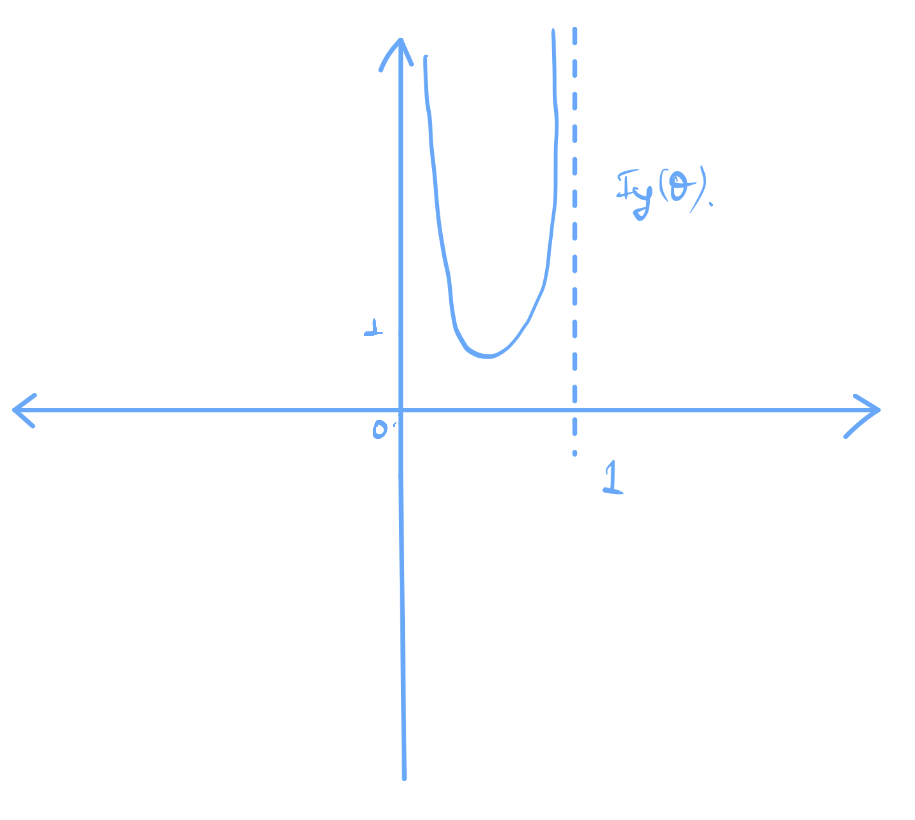
\includegraphics[width=0.8\textwidth]{crb.png}
\end{figure}

\textbf{(f)} Using CRB to directly obtain MVU is \textbf{not possible} here.
If we apply Cramer Rao theorem part (b), then $g(y) = (Y_1+Y_2)\frac{\theta}{\ln(\theta)}$ which is not a valid estimator. So, CRB is not tight in this problem.  
\end{solution}
\questionheader{Problem 3}

\begin{solution}
\[
f(y\mid \theta)=\theta e^{-\theta y}\,\mathbf{1}_{\{y\ge 0\}},\qquad
f(\theta)=\alpha e^{-\alpha\theta}\,\mathbf{1}_{\{\theta\ge 0\}}.
\]
\[
f(\theta\mid y)=\frac{f(y\mid \theta)f(\theta)}{f(y)}.
\]
Now,
\begin{align*}
f(y)
&=\int_{-\infty}^{\infty} f(y\mid \theta)f(\theta)\,d\theta\\
&=\int_0^\infty \theta e^{-\theta y}\alpha e^{-\alpha\theta}\,d\theta\\
&=\alpha\int_0^\infty \theta e^{-\theta(y+\alpha)}\,d\theta\\
&=\frac{\alpha}{(y+\alpha)^2},\qquad y\ge 0.
\end{align*}
Hence,
\begin{align*}
f(\theta\mid y)
&=\frac{\theta e^{-\theta y}\mathbf{1}_{\{y\ge0\}}\cdot \alpha e^{-\alpha\theta}\mathbf{1}_{\{\theta\ge0\}}}
{\alpha/(y+\alpha)^2\cdot \mathbf{1}_{\{y\ge0\}}}\\
&=(y+\alpha)^2\theta e^{-\theta(y+\alpha)}
\mathbf{1}_{\{y\ge0\}}\mathbf{1}_{\{\theta\ge0\}}.
\end{align*}

\textbf{3(a)}
\[
\hat\theta_{\mathrm{MAE}}(y)\ \text{is given by}
\quad
\int_{-\infty}^{\hat\theta_{\mathrm{MAE}}} f(\theta\mid y)\,d\theta
=\int_{\hat\theta_{\mathrm{MAE}}}^{\infty} f(\theta\mid y)\,d\theta
=\frac12.
\]
\[
\int_0^{\hat\theta_{\mathrm{MAE}}}(y+\alpha)^2\theta e^{-\theta(y+\alpha)}\,d\theta=\frac12.
\]
Let $T=(y+\alpha)\hat\theta_{\mathrm{MAE}}$. Then
\[
(T+1)e^{-T}=\frac12.
\]
Solving graphically, $T\approx 1.67$. Therefore
\[
\hat\theta_{\mathrm{MAE}}=\frac{1.67}{y+\alpha},\qquad y\ge0.
\]
Associated error covariance:
\begin{align*}
E_{\theta\mid y}\!\left[(\hat\theta_{\mathrm{MAE}}-\theta)^2\right]
&=\int_0^\infty (\hat\theta_{\mathrm{MAE}}-\theta)^2
(y+\alpha)^2\theta e^{-\theta(y+\alpha)}\,d\theta\\
&=\int_0^\infty\left(\hat\theta_{\mathrm{MAE}}^2+\theta^2-2\hat\theta_{\mathrm{MAE}}\theta\right)
(y+\alpha)^2\theta e^{-\theta(y+\alpha)}\,d\theta\\
&=\hat\theta_{\mathrm{MAE}}^2 (y+\alpha)^2\int_0^\infty \theta e^{-\theta(y+\alpha)}\,d\theta\\
&\quad +(y+\alpha)^2\int_0^\infty \theta^3 e^{-\theta(y+\alpha)}\,d\theta\\
&\quad -2\hat\theta_{\mathrm{MAE}}(y+\alpha)^2\int_0^\infty \theta^2 e^{-\theta(y+\alpha)}\,d\theta.
\end{align*}
Let $t=(y+\alpha)\theta$, so $d\theta=\frac{dt}{y+\alpha}$ and $\hat\theta_{\mathrm{MAE}}=\frac{1.67}{y+\alpha}$. Then
\begin{align*}
E_{\theta\mid y}\!\left[(\hat\theta_{\mathrm{MAE}}-\theta)^2\right]
&=\frac{1.67^2}{(y+\alpha)^2}\int_0^\infty t e^{-t}\,dt\\
&\quad +\frac{1}{(y+\alpha)^2}\int_0^\infty t^3 e^{-t}\,dt\\
&\quad -\frac{2(1.67)}{(y+\alpha)^2}\int_0^\infty t^2 e^{-t}\,dt\\
&=\frac{1.67^2}{(y+\alpha)^2}\Gamma(2)
+\frac{1}{(y+\alpha)^2}\Gamma(4)
-\frac{2(1.67)}{(y+\alpha)^2}\Gamma(3)\\
&=\frac{1.67^2-4(1.67)+6}{(y+\alpha)^2}\\
&=\frac{2.1089}{(y+\alpha)^2}.
\end{align*}

\textbf{3(b)}
\[
p(\theta\mid y)=(y+\alpha)^2\theta e^{-\theta(y+\alpha)}\mathbf{1}_{\{y\ge0\}}\mathbf{1}_{\{\theta\ge0\}}.
\]
\[
\hat\theta_{\mathrm{MAP}}=\arg\max_\theta p(\theta\mid y).
\]
\begin{align*}
\frac{\partial}{\partial\theta}p(\theta\mid y)
=(y+\alpha)^2\Big[
e^{-\theta(y+\alpha)}
-(y+\alpha)\theta e^{-\theta(y+\alpha)}
\Big].
\end{align*}
So,
\[
\hat\theta_{\mathrm{MAP}}=\frac{1}{y+\alpha}.
\]
Associated error covariance:
\[
E_{\theta\mid y}\!\left[(\hat\theta_{\mathrm{MAP}}-\theta)^2\right]
=\frac{1^2-4(1)+6}{(y+\alpha)^2}
=\frac{3}{(y+\alpha)^2}.
\]

\textbf{3(c)}
\[
\hat\theta_{\mathrm{MMSE}}=E(\theta\mid y)
=\int_0^\infty \theta f(\theta\mid y)\,d\theta
=\int_0^\infty \theta (y+\alpha)^2\theta e^{-\theta(y+\alpha)}\,d\theta
=\frac{2}{y+\alpha}.
\]
Associated error covariance:
\[
E_{\theta\mid y}\!\left[(\hat\theta_{\mathrm{MMSE}}-\theta)^2\right]
=\frac{2^2-4(2)+6}{(y+\alpha)^2}
=\frac{2}{(y+\alpha)^2}.
\]
I have used the form of $E_{\theta\mid y}\!\left[(\hat\theta-\theta)^2\right]$ to calculate the others also.
It has the form
\[
\frac{N^2-4N+6}{(y+\alpha)^2},
\]
where $\hat\theta=\dfrac{N}{y+\alpha}$. Since $\hat\theta_{\mathrm{MAP}}$ and
$\hat\theta_{\mathrm{MMSE}}$ are of the same form, I used this direct one-line error covariance formula.
\end{solution}

\questionheader{Problem 4 }

\begin{solution}
\textbf{(a)}
\[
p(y_i\mid \theta)=\frac{1}{\theta-1}\,\mathbf{1}_{\{1\le y_i\le \theta\}},
\qquad
p(\theta)=\frac{1}{9}\,\mathbf{1}_{\{1\le \theta\le 10\}}.
\]
\[
p(y\mid \theta)=\frac{1}{(\theta-1)^N}\,\mathbf{1}_{\{y_{(N)}\le \theta\}}.
\]
\[
p(\theta\mid y)\propto p(y\mid\theta)p(\theta)
\propto \frac{1}{(\theta-1)^N}\,\mathbf{1}_{\{y_{(N)}\le \theta\le 10\}}.
\]
We need to find mode of this.
Between $y_{(N)}$ and $10$, $\frac{1}{(\theta-1)^N}$ is monotonically decreasing.
So, mode occurs at $\theta=y_{(N)}$.
\[
\hat\theta_{\mathrm{MAP}}(y)=y_{(N)}.
\]

\textbf{(b)}
\[
\Pr(y_{(N)}\le z)=\int_1^{10}\Pr(y_{(N)}\le z\mid\theta)\,p(\theta)\,d\theta.
\]
For i.i.d.\ samples:
\[
\Pr(y_{(N)}\le z\mid\theta)=\Pr(y_1\le z\mid\theta)\cdots \Pr(y_N\le z\mid\theta)
=\left(\frac{z-1}{\theta-1}\right)^N.
\]
As $N\to\infty$:
\[
\left(\frac{z-1}{\theta-1}\right)^N\to
\begin{cases}
0,&\theta>z,\\
1,&\theta\le z.
\end{cases}
\]
Therefore
\begin{align*}
\lim_{N\to\infty}\Pr(y_{(N)}\le z)
&=\int_1^{10}\mathbf{1}_{\{\theta\le z\}}\frac{1}{9}\,d\theta\\
&=\Pr(\Theta\le z).
\end{align*}
Hence,
\[
\lim_{N\to\infty}\Pr(\hat\theta_{\mathrm{MAP}}\le z)=\Pr(\Theta\le z).
\]

\end{solution}

\questionheader{Problem 5}

\begin{solution}
\[
Y_1\sim\mathcal N(\theta_1,1),\qquad
Y_2\sim\mathcal N(\theta_1+\theta_2,1),
\]
independent. Parameter vector:
\[
\boldsymbol\theta=
\begin{bmatrix}
\theta_1\\
\theta_2
\end{bmatrix}.
\]
\[
\mathbf y=
\begin{bmatrix}
y_1\\
y_2
\end{bmatrix},\qquad
\boldsymbol\mu=
\begin{bmatrix}
\theta_1\\
\theta_1+\theta_2
\end{bmatrix},\qquad
\Sigma=
\begin{bmatrix}
1&0\\
0&1
\end{bmatrix}.
\]
\[
p_{\boldsymbol\theta}(\mathbf y)
=\frac{1}{2\pi|\Sigma|^{1/2}}
\exp\!\left(-\frac12(\mathbf y-\boldsymbol\mu)^T\Sigma^{-1}(\mathbf y-\boldsymbol\mu)\right).
\]

\textbf{(a)} Joint log-likelihood (up to constants):
\[
\ell(\theta_1,\theta_2)
 =-\frac12\Big[(y_1-\theta_1)^2+(y_2-\theta_1-\theta_2)^2\Big].
\]
Score:
\[
\frac{\partial\ell}{\partial\theta_1}=(y_1-\theta_1)+(y_2-\theta_1-\theta_2),\qquad
\frac{\partial\ell}{\partial\theta_2}=y_2-\theta_1-\theta_2.
\]
Its expectation is zero, so regularity holds.

Hessian:
\[
\frac{\partial^2\ell}{\partial\boldsymbol\theta\,\partial\boldsymbol\theta^T}
=-
\begin{bmatrix}
2&1\\
1&1
\end{bmatrix}.
\]
Therefore Fisher information matrix:
\[
\mathbf I(\boldsymbol\theta)=
\begin{bmatrix}
2&1\\
1&1
\end{bmatrix}.
\]
CRB matrix:
\[
\mathrm{CRB}=\mathbf I^{-1}=
\begin{bmatrix}
1&-1\\
-1&2
\end{bmatrix}.
\]

\textbf{(b)} Scalar CRB when estimating each parameter separately from $Y=(Y_1,Y_2)$:
\[
\operatorname{Var}(\hat\theta_1)\ge \frac{1}{2},\qquad
\operatorname{Var}(\hat\theta_2)\ge 1.
\]
(Using $-\partial^2\ell/\partial\theta_1^2=2$ and $-\partial^2\ell/\partial\theta_2^2=1$.)

\textbf{(c)} Comparison: \\
In 5(a),
\[
\operatorname{Var}(\hat\theta_1)\ge 1,\qquad
\operatorname{Var}(\hat\theta_2)\ge 2.
\]
In 5(b),
\[
\operatorname{Var}(\hat\theta_1)\ge 2,\qquad
\operatorname{Var}(\hat\theta_2)\ge 1.
\]
When jointly predicting, $\theta_1$ is present in both $Y_1$ and $Y_2$, and it gets weighted, so the variance goes down.

When jointly predicting $\hat\theta_2$, it is high since it is not sure due to presence of $\theta_1$.

\end{solution}





\end{document}
